%----------------------------------------------------------------------------------------
%	Metropolia Thesis LaTeX Template
%----------------------------------------------------------------------------------------
% License:
% This work is licensed under the Creative Commons Attribution 4.0 International License.
% To view a copy of this license, visit http://creativecommons.org/licenses/by/4.0/.
%
% However, this license apply to this template. As a template, it is supposed to be
% modified for your own needs (with your thesis content). For this reason, if you use
% this project as a template and not specifically distribute it as part of a another
% package/program, we grant the extra permission to freely copy and modify these files as
% you see fit and even to delete this copyright notice.
% In short, you are free to publish your thesis under whatever license you wish, even
% keep the all rights reserved to you.
%
% Authors:
% Panu Leppäniemi, Patrik Luoto, Mikaa Oni and Patrick Ausderau
%
% Credits:
% Panu Leppäniemi: abstract, def, cleaning,...
% Patrik Luoto: title page, abstract in Finnish, abbreviation, math,...
% Mikaa Oni: switch to biber biblatex
% Patrick Ausderau: initial version, style, table of content, bibliography, figure,
%                   appendix, table, source code listing,...
%
% Please:
% If you find mistakes, improve this template and alike, please contribute by sharing
% your improvements and/or send us your feedback there:
% https://github.com/panunu/metropolia-thesis-latex
% And of course, if you improve it, add yourself as an author.
%
% Compiler:
% Use XeLaTeX as a compiler. LuaLaTeX works too.
% Typical compilation:
% # minted require -shell-escape to run  external script.
% # -8bit avoid ^^I for tabs in minted.
% $ xelatex -shell-escape -8bit main
% # If any change in the bibliography
% $ biber main
% # If any change with the abbreviation or acronym
% $ makeglossaries main
% #Then compile again
% $ xelatex -shell-escape -8bit main
% #And if still some citation or label warnings, compile once more
% $ xelatex -shell-escape -8bit main

%----------------------------------------------------------------------------------------
%	THESIS INFO
%----------------------------------------------------------------------------------------

% All general information (main language, title, author (you), degree programme, major
% option, etc.)
% Edit the file chapters/0info.tex to change these information
\documentclass[12pt,a4paper,oneside,article]{memoir}%Do not touch this first line ;)

% Global information (title of your thesis, your name, degree programme, major, etc.)

\def\bilingual{yes}%For Finnish students, you must have 2 abstracts, one in English and one in your native language (Finnish or Swedish), so "yes", your thesis is bilingual.
%\def\bilingual{no}%For international student writing in English, only one language and one abstract.

\def\thesislang{finnish} %change this depending on the main language of the thesis.
%\def\thesislang{english} % "english" is the only other supported language currently. If someone has the swedish, please contribute!

\def\secondlang{english} %if the main language is Finnish (or Swedish), you must have 2 abstracts (one in Finnish (or Swedish) and one in English)
%\def\secondlang{finnish}
%If the main language is English and that you are native Finnish (or Swedish) speaker, you must have also abstract in your native language on top of the English one.

\author{Heikki Ketoharju} %your first name and last name

%\def\alaotsikko{Alaotsikko/Subtitle} %DISABLED, seems not to be an option with the 2018 template. If you really need it, uncomment and modify style/title.tex accordingly.

%License
%When publishing your thesis to theseus.fi, you can keep all rights reserved to you,
%or use one of the Creative Commons https://creativecommons.org/licenses/?lang=en
%This attribute will set the license in the metadata of the generated pdf.
%possible options (case sensitive):
%all (keep all rights reserved to yourself)
%by (Attribution)
%by-sa (Attribution-ShareAlike)
%by-nd (Attribution-NoDerivs)
%by-nc (Attribution-NonCommercial)
%by-nc-sa (Attribution-NonCommercial-ShareAlike)
%by-nc-nd (Attribution-NonCommercial-NoDerivs)
%Note that theseus do not accept dedication to public domain CC0
\def\thesiscopy{all}

%Finnish section, for title/abstract
\def\otsikko{Jaettua kieltä etsimässä – GraphQL-rajapinta tietomallin kohentelun
välineenä}
\def\tutkinto{Insinööri (AMK)} % change to your needs, e.g. "YAMK", etc.
\def\kohjelma{Tieto– ja viestintätekniikka}
\def\suuntautumis{Ohjelmistotuotanto}
\def\thesisfi{Insinöörityö}%was Opinnäytetyö
\def\ohjaajat{
Titteli Etunimi Sukunimi\newline
Titteli Etunimi Sukunimi
}
\def\tiivistelma{
Tämä on tiivistelmän ensimmäinen kappale. Tiivistelmän kappaleet loppuvat komentoon newline, jotta saadaan yksi tyhjä rivi aikaiseksi. \newline

Tämä on tiivistlemän toinen kappale.
}
\def\avainsanat{avainsana, avainsana}
\def\aihe{Lyhyt kuvaus opinnäytetyöstä. Max 255 merkkiä.}%for the pdf metadata/properties. If not used, empty it and also the \def\subject.

%English section, for title/abstract
\title{Your title here}
\def\metropoliadegree{Bachelor of Engineering} % change to your needs, e.g. "master", etc.
\def\metropoliadegreeprogramme{your degree programme (e.g. Information Technology)}
\def\metropoliaspecialisation{your major option (e.g. Mobile Solutions)}
\def\thesisen{Bachelor’s Thesis} % change to your need, e.g. master's
\def\metropoliainstructors{
First name Last name, Title (e.g.: Project Manager)\newline
First name Last name, Title (e.g.: Principal Lecturer)
}
\def\abstract{
Abstract content. To force newline between paragraph in the abstract, you must have both a empty line and the newline command. \newline

beginning of second paragraph\ldots
}
\def\metropoliakeywords{keyword, keyword}
\def\subject{short description of the thesis. Max 255 characters.}%for the pdf metadata/properties. If not used, empty it and also the \def\aihe.


%----------------------------------------------------------------------------------------
%	GLOBAL STYLES
%----------------------------------------------------------------------------------------

% If you need extra package, etc. modify the style/style.tex file.
% If you are using Windows OS, you will need to change default font to Arial in that
% style/style.tex file (or install Liberation Sans font to your system).
% If you are using MacOS or linux, make sure you have Liberation Sans font installed.
% Global style. Normally should not be edited.
% If you use windows OS, eventually change \setmainfont to Arial
% Check around commit https://github.com/panunu/metropolia-thesis-latex/commit/a0c15ac77bab1a52c59c517a18080938e57bf5ef
% to see how the font files were manually added (after downloading them: https://pagure.io/liberation-fonts/ )

%\usepackage[l2tabu, orthodox]{nag}%check for obsolete packages (with outdated nag package?)

%condition e.g. for adding or not space in TOC,...
\usepackage{etoolbox}
\ifdefstring{\bilingual}{yes}{
  \usepackage[\secondlang,\thesislang]{babel}% finnish (or swedish) and english
}{
  \usepackage[\thesislang]{babel}% english only
}
\usepackage{iflang}
\usepackage{amsmath}
\usepackage{amsfonts}%extra mathematical symbols
\usepackage{amssymb}
\usepackage{fontspec}
\usepackage{titlesec}
\usepackage{mathtools}%enhance the appearance of documents containing a lot of mathematics
\usepackage[amssymb]{SIunits}
\usepackage[version=3]{mhchem}
\usepackage{tikz} % mindmaps, flowcharts, piecharts, examples at http://www.texample.net/tikz/examples/
\usetikzlibrary{shapes.geometric, arrows}

\usepackage{ragged2e}
\IfLanguageName{finnish}{
  \RaggedRight%2021 template, align left and hyphennization for Finnish version
  \setlength{\RaggedRightRightskip}{0pt plus 1fil}%TODO: fix the Overfull/Underfull warnings when \RaggedRight (likely in title and abstact)
}{}
\makeatletter
  \let\@gnewline\@raggedtwoe@saved@gnewline% Restore original functionality of \newline
  \let\\\@raggedtwoe@savedcr% Restore original functionality of \\
\makeatother

%for compact list
\usepackage{enumitem}
%\usepackage{verbatim}%for block comment
%forcing single line spacing in bibliography
\DisemulatePackage{setspace}
\usepackage{setspace}
%\usepackage{eurosym}%euro symbol
%try to count
\usepackage{totcount}
%insert source code
%require -8bit -shell-escape in the xelatex compile command
%if compiling locally, consider options cachedir=minted,outputdir=~/.tex
\usepackage[newfloat]{minted}
\setminted{tabsize=2,linenos,breaklines,breaksymbolleft={\quad},baselinestretch=1}
\setmintedinline{breaklines,breakanywhere}
\usepackage[singlelinecheck=false]{caption}
%force the width of a table instead of column
\usepackage{tabularx}
\usepackage{booktabs} %why not booktabs? :3

\usepackage{csquotes}% avoid warning with babel

\usepackage{float} % For forced figure location with modifier H (\begin{figure}[H])
\usepackage{wrapfig}

% citep-macro for reference with period inside square brackets [1.]
\newcommand{\citep}[1]{
 \renewcommand\citeright{.]}
 \cite{#1}
 \renewcommand\citeright{]}
}

%set date format to D.M.YYYY
\def\pvm{\the\day.\the\month.\the\year}
%set date format to D Month YYYY
\usepackage[en,useregional=false]{datetime2}
\DTMsetup{datesep=.}
\DTMnewdatestyle{dMonthyyyy}
{%
  \renewcommand{\DTMdisplaydate}[4]{%
    \number##3 % day
    ~% separator
    \DTMenglishmonthname{##2}% month name
    ~% separator
    \number##1% year
  }%
  \renewcommand{\DTMDisplaydate}[4]{%
    \DTMdisplaydate{##4}{##3}{##2}{##1}%
  }%
}
\DTMsetdatestyle{dMonthyyyy}
\date{\today}

\newcommand\tn[1]{\textnormal{#1}} %use \tn instead of \textnormal
\newcommand\reaction[1]{\begin{equation}\ce{#1}\end{equation}} %\reaction{} for chemical reactions

%NORMAL TEXT
%all text, title, etc. in the same font: Arial
%NOTE: fontname is case-sensitive
\setmainfont[Scale=0.98]{Liberation Sans}
%line space
\linespread{1.46}
\AtBeginEnvironment{tabular}{\singlespacing}
%\doublespacing
%margin
%geometry moved after hyperref
\setlength{\parindent}{0pt} %first line of paragraph not indented
\setlength{\parskip}{16.5pt} %one empty line to separate paragraph
%list with small line space separation
\tightlists
\setlist[itemize]{before=\singlespacing,itemsep=6pt,leftmargin=63pt,labelsep=22pt,topsep=1.5pt,partopsep=0pt,after=\vspace{-22pt}\newline}
\setlist[enumerate]{before=\singlespacing,itemsep=6pt,leftmargin=63pt,labelsep=22pt,topsep=1.5pt,partopsep=0pt,after=\vspace{-22pt}\newline}

%IMAGE - FIGURE
%the figures should be placed in the "illustration" folder
\graphicspath{{illustration/}}
%figure number without chapter (1.1, 1.2, 2.1) to (1, 2, 3)
\counterwithout{figure}{chapter}
%border around images
\setlength\fboxsep{0pt}
\setlength\fboxrule{0.5pt}
%space after figure caption (and other float elements)
\setlength{\belowcaptionskip}{-7pt}
\setlength{\intextsep}{16.5pt}%space around floats
\AtBeginEnvironment{table}{\addvspace{16.5pt}}

%TABLE
\counterwithout{table}{chapter}

%SOURCE CODE
\newenvironment{code}{\captionsetup{type=listing}}{}
\IfLanguageName{finnish}{\SetupFloatingEnvironment{listing}{name=Koodiesimerkki}}{}%was Listaus
%\counterwithout{lstlisting}{chapter}
%moved after begin document, otherwise does not compile

%TOC
%change toc title
\IfLanguageName{finnish}{\addto{\captionsfinnish}{\renewcommand*{\contentsname}{Sisällys}}}{}
%remove dots
\renewcommand*{\cftdotsep}{\cftnodots}
%chapter title and page number not in bold
\renewcommand{\cftchapterfont}{\normalfont}
\renewcommand{\cftchapterpagefont}{\normalfont}
%sub section in toc
\setcounter{tocdepth}{2}
%subsection numbered
\setcounter{secnumdepth}{2}
\renewcommand{\tocheadstart}{\vspace*{-33.5pt}}
\renewcommand{\printtoctitle}[1]{\fontsize{13.5pt}{13.5pt}\bfseries #1\vspace*{-4pt}}
%\renewcommand{\aftertoctitle}{\vspace*{-22pt}\afterchaptertitle}
%spacing after a chapter in toc
\preto\section{%
  \ifnum\value{section}=0\addtocontents{toc}{\vskip11pt}\fi
}
%spacing after a section in toc
\renewcommand{\cftsectionaftersnumb}{\vspace*{-3pt}}
%spacing after a subsection in toc
\renewcommand{\cftsubsectionaftersnumb}{\vspace*{-1pt}}
%appendix in toc with "Appendix " + num
\IfLanguageName{finnish}{
  \renewcommand*{\cftappendixname}{Liite\space}
  \renewcommand{\appendixtocname}{Liitteet}
}{\renewcommand*{\cftappendixname}{Appendix\space}}
%appendix header
\IfLanguageName{finnish}{\def\appname{Liite\space}}{\def\appname{Appendix\space}}

%TITLES
%chapter title
%\clearforchapter{\clearpage}
\titleformat{\chapter}
{\fontsize{14pt}{14pt}\bfseries\linespread{1}}%\clearpage
{\thechapter}{.5cm}{}
\titlespacing*{\chapter}{0pt}{21.5pt}{.5pt}
\titleformat{\section}
{\fontsize{13.5pt}{13.5pt}\normalfont}
{\thesection}{.5cm}{}
\titlespacing*{\section}{0pt}{9pt}{0pt}
\titleformat{\subsection}
{\fontsize{12.7pt}{12.7pt}\normalfont}
{\thesubsection}{.5cm}{}
\titlespacing*{\subsection}{0pt}{11pt}{0pt}


%QUOTE
\renewenvironment{quote}
{\list{}{\rightmargin=0pt\leftmargin=2.2cm\topsep=-14pt}%
  \item\relax\singlespacing}%\fontsize{10pt}{10pt}
    {\vspace{8pt}\endlist}

%BIBLIOGRAPHY
%TODO: toggle for Harward v.s. Vancouver
\usepackage[
backend=biber,
bibencoding=utf8,%
citetracker=true,%
isbn=false,%
doi=false,%
url=true,%
usetranslator=true,%
bibstyle=ext-authoryear,%
citestyle=numeric-comp,%
sorting=none,%
sortcites=true,%
block=none,%
terseinits=false,%
giveninits=false,%
maxbibnames=99,%
]{biblatex}

\setlength{\bibitemsep}{11pt}
\setlength{\biblabelsep}{1cm}%with 1cm horizontal gap

\makeatletter
\RequireBibliographyStyle{numeric}
\makeatother

% set right format
\renewcommand*{\multicitedelim}{;\space}
\renewcommand*{\multinamedelim}{;\space}
\renewcommand*{\finalnamedelim}{~\&\space}
\DeclareFieldFormat{biblabeldate}{#1}
\DeclareDelimFormat[bib]{nameyeardelim}{\addperiod\space}
%\DeclareNameAlias{sortname}{last-first} % deprecated
\DeclareNameAlias{default}{family-given}
\DeclareFieldFormat{labelnumberwidth}{#1} % remove () from label number
\DeclareFieldFormat{title}{#1} % normal font for title
\DeclareFieldFormat{citetitle}{#1}
\DeclareFieldFormat{journaltitle}{#1} % remove underline
\DeclareFieldFormat*{url}{%
\ifentrytype{online}{\IfLanguageName{finnish}{Verkkoaineisto}{Online}\addperiod\space}{}%
\ifentrytype{video}{Video\addperiod\space}{}%
\textless\url{#1}\textgreater\addperiod
} % you can modify how to url looks here
%TODO: remove leading 0 for day and month for Finnish dates
\DeclareFieldFormat{urldate}{\space\bibstring{urlseen}\space#1} % remove () from date
%try set translation to biblio
\DefineBibliographyStrings{english}{%
    urlfrom = {available at},%
    urlseen = {Visited on},%
    fromenglish = {from English},%
    fromfinnish = {from Finnish},%
    fromgerman = {from German},%
    fromjapanese = {from Japanese},%
}
\DefineBibliographyStrings{finnish}{%
  %  urlfrom={Linkki: },%
    urlfrom = {},%
    urlseen = {Luettu},%
    fromjapanese = {japanista},%
    fromenglish = {englannista},%
    fromfinnish = {suomesta},%
    fromgerman = {saksasta},%
}
{
  %new cite command: "Vancouver Short"
  \DeclareCiteCommand{\citeVS}
    {\usebibmacro{prenote}}
    {\usebibmacro{author}, \usebibmacro{title}}
    {\multicitedelim}
    {\usebibmacro{postnote}}

  % new cite command: "Vancouver Short Collection" - necessary when referencing whole collections.
  \DeclareCiteCommand{\citeVSc}
    {\usebibmacro{prenote}}
    {\usebibmacro{editor}, \usebibmacro{title}}
    {\multicitedelim}
    {\usebibmacro{postnote}}
}

\addbibresource{biblio.bib}% for biblatex you need out \printbibliography too

%count the appendices (since the chapter counter is reset after \appendix).
%! require to complie 2 times
\regtotcounter{chapter}

% metadata (title, author, lang,...) for accessibility, etc.
\usepackage{hyperref}
\usepackage{hyperxmp}
\def\isolang{\IfLanguageName{finnish}{fi}{en}} %iso code (based on main language)
\ifdefstring{\thesiscopy}{all}{%
    \def\copyen{Copyright \textcopyright\ \the\year{}, \theauthor}
    \def\copyfi{Kaikki oikeudet pidätetään.  \textcopyright\ \the\year{}, \theauthor}
  }{%
    \usepackage[type={CC},modifier={\thesiscopy},version={4.0},]{doclicense}
    \def\copyen{\thetitle\ \textcopyright\ \the\year{} by \theauthor\ is licensed under \doclicenseLongNameRef}
    \def\copyfi{\otsikko\ \textcopyright\ \the\year{}, jonka tekijä on \theauthor, on lisensoitu \doclicenseLongNameRef}
}
\hypersetup{%
  pdfdisplaydoctitle,
  %breaklinks=true,%searching for overfull warnings
  pdfencoding=auto,
  bookmarksdepth=subsection,
  unicode=true,
  keeppdfinfo=true,
  pdflang={\isolang},
  pdfmetalang={\isolang},
  pdftitle={\IfLanguageName{finnish}{\otsikko}{\thetitle}},
  pdfkeywords={\IfLanguageName{finnish}{\avainsanat}{\metropoliakeywords}},
  pdfcopyright={\IfLanguageName{finnish}{\copyfi}{\copyen}},
  pdfsubject={\IfLanguageName{finnish}{\aihe}{\subject}},
}

\ifdefstring{\bilingual}{yes}{%metadata (title and copyright) in multiple language
  \XMPLangAlt{\IfLanguageName{finnish}{en}{fi}}{%
    pdftitle={\IfLanguageName{finnish}{\thetitle}{\otsikko}},
    pdfcopyright={\IfLanguageName{finnish}{\copyen}{\copyfi}},
    pdfsubject={\IfLanguageName{finnish}{\subject}{\aihe}},
  }
}{}
\urlstyle{same}

%moved after hyperred as can cause conflicts
\usepackage{pdfcomment}%try the alt text for graphics
\usepackage{accsupp}
\newcommand{\AltText}[2]{\BeginAccSupp{method=pdfstringdef,unicode,Alt={{#1}}}\pdftooltip{{#2}}{{#1}}\EndAccSupp{}}

\usepackage[top=2.5cm, bottom=3cm, left=4cm, right=2cm, nofoot]{geometry}

\usepackage{pgfplots} %simple plots etc
\pgfplotsset{compat=1.16}
\usepackage{pgfplotstable}

% Abbreviations, acronym and glossary, in case of bug, remove temporary the noredefwarn
\usepackage[acronym,toc,nonumberlist,section=chapter,noredefwarn]{glossaries}%xindy,%toc, ,nomain
\newglossarystyle{mystyle}{%
  \setglossarystyle{list}% base this style on the list style
  \renewcommand*{\glossentry}[2]{%
  \item[\glsentryitem{##1}%
    \glstarget{##1}{\glossentryname{##1}:}]
  \glossentrydesc{##1}\glspostdescription\space ##2}
}
\setglossarystyle{mystyle}

\renewcommand*{\glsclearpage}{}

% Normally, you do not need to modify the title style. It's content comes from the
% chapters/0info.tex file.
\input{style/title.tex}

%----------------------------------------------------------------------------------------
%	ABBREVIATION AND GLOSSARY
%----------------------------------------------------------------------------------------

% Add/edit all your acronyms, abbreviations, glossary entries, etc. definitions in
% chapters/0abbr.tex file.
% You can have as many as you wish. Only the ones you use in your text (inserted with
% \gls{} command) will print in the Glossary/Lyhenteet.
% Generate the glossary
\makeglossaries

% Acronyms, abbreviations, etc.

\newacronym{lamp}{LAMP}{LAMP (Linux, Apache, MySQL, PHP)}
\newacronym{orm}{ORM}{Object-relational mapper, oliot tietokantatauluiksi muuntava teknologia}
\newacronym{sql}{SQL}{Structured Query Language}
\newacronym{io}{I/O}{Input/Output}
\newacronym{ram}{RAM}{Random Access Memory}
\newacronym{php}{PHP}{Hypertext Preprocessor}
\newacronym{wysiwym}{WYSIWYM}{What You See Is What You Mean}
\newacronym{isbn}{ISBN}{International Standard Book Number}
\newacronym{url}{URL}{Uniform Resource Locator}
\newacronym{doi}{DOI}{Digital Object Identifier}


\newacronym{html}{HTML}{HyperText Markup Language}


% Glossary entries
\newglossaryentry{ddd}{
  name={Sovellusaluevetoinen suunnittelu},
  text={sovellusaluevetoinen suunnittelu},
  description={Menetelmä, jossa ohjelmistoa kehitetään läheisessä yhteistyössä sovellusalueen asiantuntijoiden kanssa. (myös: Liiketoimintavetoinen suunnittelu.) Engl. Domain Driven Design}
  }
\newglossaryentry{domain}{
  name={Sovellusalue},
  text={sovellusalue},
  description={Erityisala, jota sovellus käsittelee. Esimerkiksi pankkitoiminta tai vähittäiskauppa. myös: liiketoimintataso}
}

\newglossaryentry{crunching}{
  name={Tiedon rouhinta},
  text={tiedon rouhinta},
  description={Prosessi, jossa tunnistetaan sovellusalan erityiskäsitteitä ohjelmoijan ja sovellusalueen asiantuntijan välisen kommunikaation avulla. Engl. Knowledge crunghing}
  }
\newglossaryentry{dsl}{
  name={Täsmäkieli},
  text={täsmäkieli},
  description={Erityisalaan liittyvä formaali kieli. Esimerkiksi ohjelmointi- tai kuvauskieli. Engl. Domain-Specific language}
  }
\newglossaryentry{ubilang}{
  name={Kaikenkattava kieli},
  text={kaikenkattava kieli},
  description={Kokoelma käsitteitä ja sanastoa, joiden avulla ohjelmoijat ja sovellusalueen asiantuntijat keskustelevat kehitettävästä ohjelmistosta. Muotoutuu tiedon rouhintaprosessin tuloksena. Engl. Ubiquitous language}
  }
\newglossaryentry{domainmodel}{
  name={Sovellusaluemalli},
  text={sovellusaluemalli},
  description={Käsitteistä ja niiden välisistä suhteista koostuva, ohjelmakoodin muotoon kaapattava malli käsiteltävästä sovellusalueesta. Engl. Domain Model}
  }
\newglossaryentry{domainlayer}{
	name={Liiketoimintalogiikan taso},
	text={liiketoimintalogiikan taso},
	description={Ohjelmiston sisäinen osa, joka pitää sisällään liiketoimintaan liittyvän ohjelmalogiikan. Engl. Domain layer},
}
\newglossaryentry{entity}{
	name={Yksilötyyppi},
	text={yksilötyyppi},
	description={Ohjelmassa esiintyvä olio, jolla on identiteetti. Esimerkiksi yksittäinen asiakas tai lasku. Engl. Entity},
}
\newglossaryentry{deepermodel}{
  name={Syvempi malli},
  text={syvempi malli},
  description={Sovellusaluevetoisen suunnittelun myötä parantunut sovellusaluemalli. Syvempi malli tavoittaa aiempaa paremmin sovellusalan perimmäisen luonteen. Engl. Deeper Model}
}
\newglossaryentry{hakurakenne}{
  name={Assosiaatiotaulu},
  text={assosiaatiotaulu},
  description={Engl. Map. suom. myös {\em hakurakenne\/} ja {\em sanakirja\/}. Tietorakenne, joka sisältää joukon avain-arvo -pareja}
}

\newglossaryentry{rest}{
  name={REST},
  text={REST},
  description={Representational State Transfer. Arkkitehtoninen tyyli rajapintojen määrittelemiseen etenkin Web-sovelluksissa}
}

\newglossaryentry{graphql}{
  name={GraphQL},
  text={GraphQL},
  description={Facebookin kirjoittama kyselykieli, joka esittää manipuloitavan datan olioverkkona}
}

\newglossaryentry{http}{
  name={HTTP},
  text={HTTP},
  description={Hypertext Transfer Protocol. Webin perusprotokolla, jota käytetään hypertekstidokumenttien siirtoon}
}

\newglossaryentry{verkko}{
  name={Verkko},
  text={verkko},
  description={Tietorakenne, joka koostuu solmuista ja kaarista}
}

\newglossaryentry{domainexpert}{
  name={Alan asiantuntija},
  text={alan asiantuntija},
  description={Sovellusalueen esimerkiksi työnsä puolesta hyvin tunteva henkilö}
}

\newglossaryentry{kulkusuunta}{
  name={Kulkusuunta},
  text={kulkusuunta},
  description={Olioita yhdistävän kytköksen suunta}
}

\newglossaryentry{puhdasfunktio}{
  name={Puhdas funktio},
  text={puhdas funktio},
  description={Funktio, jonka palauttama tulos riippuu vain sen saamien parametrien arvoista. Puhdas funktio ei aiheuta sivuvaikutuksia esimerkiksi tulostamalla ruudulle tai tallentamalla tiedostoon}
}

\newglossaryentry{tyyppi}{
  name={Tyyppi},
  text={tyyppi},
  description={Lausekkeeseen sidottu määritys lausekkeen palauttaman arvon tietotyypistä. Esimerkiksi kokonaisluku tai merkkijono}
}

\newglossaryentry{aggregate}{
  name=Aggregaatti,
  text=aggregaatti,
  description={Useiden olioiden kokoelma, jolla on yksi juuriolio. Käsitellään ohjelmalogiikassa yhtenä kokonaisuutena.}
}
\newglossaryentry{repository}{
  name=Repositorio,
  text=repositorio,
  description=Rajapinta tiedon tallennusvälineeseen
}
\newglossaryentry{factory}{
  name=Tehdas-olio,
  text=tehdas-olio,
  description={Olio, joka vastaa toisten olioiden luomisesta}
}



%----------------------------------------------------------------------------------------
%	DOCUMENT STARTS HERE...
%----------------------------------------------------------------------------------------

\begin{document}
\IfLanguageName{finnish}{
}{
  \raggedright%2021 template, align left, no hyphennization for English version
}
\counterwithout{listing}{chapter}

%----------------------------------------------------------------------------------------
%	TITLE PAGE
%----------------------------------------------------------------------------------------

\input{style/title_headers.tex}
\maketitle
\newpage

%----------------------------------------------------------------------------------------
%	ABSTRACT / Tiivistelmä
%----------------------------------------------------------------------------------------

% If you are international student writing in English, ignore the Finnish abstract.
% If you are Finnish citizen, you must have 2 abstracts, one in Finnish (or Swedish
% depending on your mother tongue) and one in English regardless of the main language of
% your thesis. Normally, you do not need to modify the abstract style. It's content comes
% from the chapters/0info.tex file.
\ifdefstring{\bilingual}{no}{%
    \input{style/abstract_en.tex}
    }{%
    \IfLanguageName{finnish}{%order of abstracts based on main language and spacing hell
        % Abstract in Finnish
% Normally, you should not edit this file. Everything comes from chapter/0info.tex

\pagestyle{empty} %remove page number
\newgeometry{top=1.5cm,left=4cm,right=.5cm}
\begin{otherlanguage}{finnish}
{\large\textbf{Tiivistelmä}}
{\renewcommand{\arraystretch}{1.1}
  \begin{tabular}{@{}p{4.7cm} >{\raggedright\arraybackslash}p{10.8cm}@{}}
  Tekijä: & \makeatletter\@author\makeatother
  \\
  Otsikko: & \otsikko
  \\
  Sivumäärä: & \pageref*{LastPage} sivua
  \\
  Aika: & \pvm
  \\[6.5mm]
  Tutkinto: & \tutkinto
  \\
  Tutkinto-ohjelma: & \kohjelma
  \\
  Ammatillinen pääaine: & \suuntautumis
  \\
  Ohjaajat: & \ohjaajat
  \\[11mm]
  \cmidrule[.7pt](l{-.15em}r{5.5em}){1-2}
  \multicolumn{2}{>{\raggedright}p{15.5cm}}{
  \vspace{.2mm}
  \tiivistelma
  }
  \\
  \\
  Avainsanat: & \avainsanat
  \\
\end{tabular}
}
\end{otherlanguage}
\restoregeometry
\clearpage


        % Abstract in English
% Normally, you should not edit this file. Everything comes from chapter/0info.tex

\pagestyle{empty} %remove page number
\newgeometry{top=1.77cm,left=4cm,right=.5cm}
\begin{otherlanguage}{english}
{\large\textbf{Abstract}}
{\renewcommand{\arraystretch}{1.1}
  \begin{tabular}{@{}p{4.7cm} >{\raggedright\arraybackslash}p{10.8cm}@{}}
  Author: & \makeatletter\@author\makeatother
  \\
  Title: & \makeatletter\@title\makeatother
  \\
  Number of Pages: & \pageref*{LastPage} pages
  \\
  Date: & \makeatletter\thedate\makeatother
  \\[6.5mm]
  Degree: & \metropoliadegree
  \\
  Degree Programme: & \metropoliadegreeprogramme
  \\
  Professional Major: & \metropoliaspecialisation
  \\
  Supervisors: & \metropoliainstructors
  \\[9mm]
  \cmidrule[.7pt](l{-.15em}r{5.5em}){1-2}
  \\
  \multicolumn{2}{>{\raggedright}p{15.5cm}}{
    \abstract
  }
  \\
  \\
  Keywords: & \metropoliakeywords
  \\
\end{tabular}
}
\end{otherlanguage}
\restoregeometry
\clearpage


        }{
        \input{style/abstract_en.tex}
        % Abstract in Finnish
% Normally, you should not edit this file. Everything comes from chapter/0info.tex

\pagestyle{empty} %remove page number
\newgeometry{top=2.04cm,left=4cm,right=.5cm}
\begin{otherlanguage}{finnish}
{\large\textbf{Tiivistelmä}}
{\renewcommand{\arraystretch}{1.1}
  \begin{tabular}{@{}p{4.7cm} >{\raggedright\arraybackslash}p{10.8cm}@{}}
  Tekijä: & \makeatletter\@author\makeatother
  \\
  Otsikko: & \otsikko
  \\
  Sivumäärä: & \pageref*{LastPage} sivua
  \\
  Aika: & \pvm
  \\[6.5mm]
  Tutkinto: & \tutkinto
  \\
  Tutkinto-ohjelma: & \kohjelma
  \\
  Ammatillinen pääaine: & \suuntautumis
  \\
  Ohjaajat: & \ohjaajat
  \\[4mm]
  \cmidrule[.7pt](l{-.15em}r{5.5em}){1-2}
  \\
  \multicolumn{2}{>{\raggedright}p{15.5cm}}{
  \tiivistelma
  }
  \\
  \\
  Avainsanat: & \avainsanat
  \\
\end{tabular}
}
\end{otherlanguage}
\restoregeometry
\clearpage


    }
}
%----------------------------------------------------------------------------------------
%	License? Acknowledgement?
%----------------------------------------------------------------------------------------

% Uncomment next line and edit chapters/0license.tex if you want license in your thesis.
%% License of your thesis
% If you wish to explain what it means. When you publish your thesis in https://theseus.fi
% you will be able to choose between some Creative Commons licenses
% https://creativecommons.org
% Adapt this example text to your taste.
% This would also be the right place to explain the license you choose for the code you
% produced for your thesis.

\pagestyle{empty}
\chapter*{Licenses}
\ifdefstring{\thesiscopy}{all}{}{%
  \begin{wrapfigure}{r}{0.3\textwidth}
    \vspace{-20pt}
    \doclicenseImage
  \end{wrapfigure}
 }
\IfLanguageName{finnish}{\copyfi}{\copyen}

That means:

%adapt to the license you choose. In this example: https://creativecommons.org/licenses/by-sa/4.0/deed.en
\textbf{You are free to:}
\begin{itemize}
\item Share \textemdash copy and redistribute the material in any medium or format
\item Adapt \textemdash remix, transform, and build upon the material
\end{itemize}

\textbf{Under the following terms:}
\begin{itemize}
\item \ccAttribution~ Attribution \textemdash You must give appropriate credit, provide a link to the license, and indicate if changes were made. You may do so in any reasonable manner, but not in any way that suggests the licensor endorses you or your use.
\item \ccShareAlike~ ShareAlike \textemdash If you remix, transform, or build upon the material, you must distribute your contributions under the same license as the original.
\item No additional restrictions \textemdash You may not apply legal terms or technological measures that legally restrict others from doing anything the license permits.
\item Any of the above conditions can be waived if you get my permission
\end{itemize}

%Eventually consider few words why you choose such license? E.g. something like:

Työmallista laatimani havainnekuva käyttää kahta vektorimuotoista kuvaa, joiden
tekijä tulee mainita.
Sivustolta Vecteezy
Doctor and surgeon wearing medical masks käyttäjältä jemastock
Female Developer Vector käyttäjältä biggorilla 298

\clearpage


% Uncomment next line and edit chapters/0acknowledgement.tex if you want acknowledgements.
%\input{chapters/0acknowledgement.tex}

%----------------------------------------------------------------------------------------
%	TABLE OF CONTENTS
%----------------------------------------------------------------------------------------

\input{style/toc.tex}

%list of figure, tables would come here if relevant?

%----------------------------------------------------------------------------------------
%	Lyhenteet / Abbreviation
%----------------------------------------------------------------------------------------

% If you don't use abbreviations/glossary, remove the following line.
% Abbreviation and Glossary
% Normally, you don't have to modify this file. Your abbreviations, etc. goes in
% ../chapters/0abbr.tex file.

\begin{singlespacing}

	% \gsladdall%would add all terms even if not used in your text.
	\addtocontents{toc}{\cftpagenumbersoff{chapter}}
	{
		\vspace{-.46cm}
		\titleformat{\section}
		{\fontsize{13.5pt}{13.5pt}\bfseries\normalfont}
		{\thesection}{.5cm}{}
		\renewcommand*{\glossarypreamble}{\vspace{.7\baselineskip}}
		%Adapt labelwidth (sorry for the ugly hack)
		\setlist[description]{leftmargin=!, labelwidth=4em, before=\doublespacing}
		\IfLanguageName {finnish} {
			\printacronyms[title=Lyhenteet, nogroupskip]
			}{
			\printacronyms[title=List of Abbreviations, nogroupskip]
		}
		\setlist[description]{leftmargin=!, labelwidth=10em}
		\vspace{1cm}
		\printglossary[]
		\setlist[description]{style=standard} % reset settings back to default
	}
	\addtocontents{toc}{\cftpagenumberson{chapter}}
\end{singlespacing}

\clearpage


%----------------------------------------------------------------------------------------
%	CONTENT
%----------------------------------------------------------------------------------------

\input{style/content.tex}%reset page number to 1, etc.

% Thesis content if you strictly follow the "Final Year Project guide". Of course, you
% can adapt to your specific needs (add more chapter, rename them, etc.).
% Introduction

\chapter{Johdanto}

Pitkäikäinen, jatkuvasti kehitetty ohjelma mutkistuu herkästi. Jos kehitystiimi
ei pidä varaansa, alun perin yksinkertaisesta ja selkeästä ohjelmakoodista ja suoraviivaisesta tietorakenteesta kasvaa hankalasti hallittava kokonaisuus.

Sotkuiseenkin ohjelmistoon voi kuitenkin saada selvyyttä taitavalla kohentelulla
ja kehittämisellä. Kun toimintoja alkaa jakaa osiin, ja rakentaa osien välille
selkeitä nivelkohtia, avautuu mahdollisuus tehdä hedelmällisiä parannuksia.

Web-sovelluksessa eräs merkittävimpiä nivelkohtia on sovelluksen käyttöliittymän
ja logiikkaosan välinen HTTP-rajapinta. Tässä insinöörityössä tarkastellaan,
voiko tämän rajapinnan uudistamisen kanssa yhtä aikaa myös kohentaa ohjelmiston sisäistä logiikkaa.

Työ tehdään ohjelmistopalveluyritys Nordhealth Oy:n tilauksesta.
 
\section{Nordhealth Oy lyhyesti}


Nordhealth Oy on vuonna 2001 perustettu ohjelmistopalveluyritys, joka tekee toiminnanohjausjärjestelmiä kahdelle eri toimialalle: Provet Cloud -järjestelmää eläinlääkäriklinikoille ja Diarium-järjestelmää terapeuteille. Molemmat järjestelmät ovat web-pohjaisia sovelluksia. Niitä käytetään kirjautumalla web-selaimen kautta. (Tästä puuttuu perustietoja, kuten työntekijöiden määrä, liikevaihto tms.)

Nordhealthia voisi luonnehtia tyypilliseksi ohjelmistoalan yritykseksi: se tekee
erityisalalle suunnattua toiminnanohjausjärjestelmää. Alunperin järjestelmät
ovat olleet työpöytäsovelluksia, ja siitä Nordhealth on muuntanut ne
LAMP-alustalla toimiviksi web-sovelluksiksi. Kun Web on kehittynyt, on otettu
suunnaksi sovellusten siirtäminen julkiseen pilveen, ja käyttöliittymän
rakentaminen erilliseksi yhden sivun JavaScript-sovellukseksi.

Diarium on Nordhealthin kahdesta järjestelmästä vanhempi. Se on suunnattu terapeuteille: fysio-, toiminta-, puhe- ja psykoterapeuteille. Järjestelmä on laajentunut yksinkertaisesta potilaskortistojärjestelmästä suurenkin terapia-alan yrityksen tarpeita vastaavaksi toiminnanohjausjärjestelmäksi, ja se on lisäksi myös Valviran tarkoittama A-luokan potilastietojärjestelmä. Diariumia käyttävä terapeutti voi siis lähettää käyntikirjaukset potilastiedon sähköiseen Kanta-rekisteriin.

\section{Insinöörityön tavoite}

Työn tavoitteena on analysoida pientä osaa Diariumin tietomallista, ja etsiä
parempia tapoja sen toteuttamiseen. Diariumin HTTP-rajapintaa halutaan muista
syistä kehittää, ja tämä tarjoaa työni pääkysymyksen: onko ohjelmiston
tietomallia mahdollista kehittää rakentamalla GraphQL-rajapinta?

GraphQL on teknologiana uusi ja erilainen verrattuna vanhaan HTTP REST
-rajapintaan. Tarvitaan siis hyviä perusteita siihen siirtymiselle.

Taustateoksena työssä käytän Eric Evansin kirjaa Doman Driven Design.

Työn tuloksena en ajattele syntyvän valmista ja parempaa tietomallia, vaan
pikemminkin prosessi tietomallin kehittämiseksi rajapinnan uusimisen ohella.
% uncomment what you need.
%\input{chapters/projectSpec.tex}
%\vspace{21.5pt}

\hypertarget{tyuxf6n-eteneminen}{%
\chapter{Työn eteneminen}\label{tyuxf6n-eteneminen}}

Tähän tulee laajempi kuvaus, kunhan päiväkirja on saatu valmiiksi

\hypertarget{ubiquitous-language-kuxe4ytuxe4nnuxf6ssuxe4}{%
\section{Ubiquitous Language
käytännössä}\label{ubiquitous-language-kuxe4ytuxe4nnuxf6ssuxe4}}

Pitäessäni suunnittelukokouksia yhdessä tuoteomistajan kanssa, pyrin
koko ajan kuuntelemaan tarkalla korvalla, minkälaisia sanoja käytimme.
Tällä tavoin onnistuin nappaamaan joitain tärkeitä käsitteitä, joita
pystyi käyttämään mallin pohjana. Toisen kokouksemme aikana esiin
noussut \textbf{Laskutusperuste} oli juuri tällainen käsite.

Eric Evans mainitsee, että \textbf{Kaikenkattavan kielen} rakentamisessa
oleellista on löytää sanat, joita alan asiantuntijat käyttävät.

\hypertarget{kuxe4sitekarttojen-ja-graphql-skeeman-yhteys}{%
\section{Käsitekarttojen ja GraphQL-skeeman
yhteys}\label{kuxe4sitekarttojen-ja-graphql-skeeman-yhteys}}

Olin yllättynyt, miten täsmällisesti piirtämäni käsitekartat oli
mahdollista ilmaista GraphQL-skeeman avulla. Olioiden suhteet siirtyivät
vaivattomasti skeeman sisälle hierarkioiksi.

%\vspace{21.5pt}

\hypertarget{teoria}{%
\chapter{Teoria}\label{teoria}}

Keskeisten käsitteiden esittely

\hypertarget{domain-driven-design}{%
\section{Domain Driven Design}\label{domain-driven-design}}

(Sovellusalakeskeinen suunnittelu) (Liiketoimintavetoinen suunnittelu)

\hypertarget{knowledge-crunching}{%
\subsection{Knowledge crunching}\label{knowledge-crunching}}

\hypertarget{ubiquitous-language}{%
\subsection{Ubiquitous Language}\label{ubiquitous-language}}

\hypertarget{mallin-ilmaiseminen-ohjelmistossa}{%
\subsection{Mallin ilmaiseminen
ohjelmistossa}\label{mallin-ilmaiseminen-ohjelmistossa}}

\begin{itemize}
\tightlist
\item
  Domain-malli on ohjelmistossa omana erillisenä kerroksenaan, puhtaasti
  ja erillään muista.
\item
  Entity - entiteetti, eli olio, jolla on identiteetti
\item
  Assosiaatio, eli kulkusuunta
\end{itemize}

Pohdintaa: - Evans suosittaa kerroksittaista arkkitehtuuria, ja
erillistä kerrosta, jossa Domain-malli elää. Luonteva paikka tälle voisi
olla GraphQL-rajapinnan takana.

\hypertarget{graphql}{%
\section{GraphQL}\label{graphql}}

\hypertarget{tyyppijuxe4rjestelmuxe4}{%
\subsection{Tyyppijärjestelmä}\label{tyyppijuxe4rjestelmuxe4}}

GraphQL-rajapinta koostuu tyypeistä

\hypertarget{query-ja-mutation}{%
\subsection{Query ja Mutation}\label{query-ja-mutation}}

Rajapintaan voi tehdä queryjä - nämä ovat ikäänkuin sisäänmenoaukkoja,
joiden kautta oliorakenteita voi pyytää Mutation - toiminto datan
muuntelemiseen. Myös tämä palauttaa dataa

\hypertarget{skeema}{%
\subsection{Skeema}\label{skeema}}

Rajapinnan tyypit, niille tehtävät kyselyt ja mutaatiot kuvataan
skeemassa, GraphQL-kielen avulla.

-Pohdintaa: Tämä skeema on varmaankin keskeinen nivelkohta Domain Driven
Designin kanssa.

%\input{chapters/solution.tex}
%\input{chapters/conclusion.tex}
\vspace{21.5pt}

\hypertarget{puxe4ivuxe4kirja-insinuxf6uxf6rityuxf6stuxe4}{%
\chapter{Päiväkirja
insinöörityöstä}\label{puxe4ivuxe4kirja-insinuxf6uxf6rityuxf6stuxe4}}

\hypertarget{viikko-1}{%
\section{Viikko 1}\label{viikko-1}}

Pidin palaverin Pasin ja Lauran kanssa. Sovimme taajaksi aihealueeksi
Diariumin laskutuksen. Varsinainen ongelma, johon keskitytään, on usean
maksajan laskut. Sanotaan, että hoitokäynnin lasku jaetaan kahtia,
asiakkaan maksamaan ja Kelan maksamaan osuuteen. Asiakkaan osuus
laskutetaan asiakkaalta, Kelan osuus taas Kelalta. Mutta Kela kieltäytyy
korvaamasta kyseistä käyntiä. Kirjanpidollisesti Kelalle lähetetty lasku
täytyy siis hyvittää. Mutta asiakkaalle lähetettyä laskua taas ei voi
hyvittää. Ja lisäksi täytyy voida ohjelmassa näyttää, että osa laskusta
on edelleen avoin.

Lauran kanssa yhdessä alettiin keskustella laskutuksesta. Laura näytti,
miten Diariumissa laskuttamisen logiikka toimii, ja piirsin
tussitaululle esimerkkejä, miten logiikka voisi toimia.

Käytin yksinkertaista notaatiota, jossa merkitsin asioita laatikoilla,
ja niiden välisiä yksi moneen -suhteita.

Piirsin aluksi käynnin. Niitä voi kuulua laskulle yksi tai useampia.
Laskut voidaan koostaa koontilaskuiksi. Koontilaskuja tai niiden osia
taas voidaan hyvittää luomalla hyvityslaskuja.

\begin{figure}
\centering
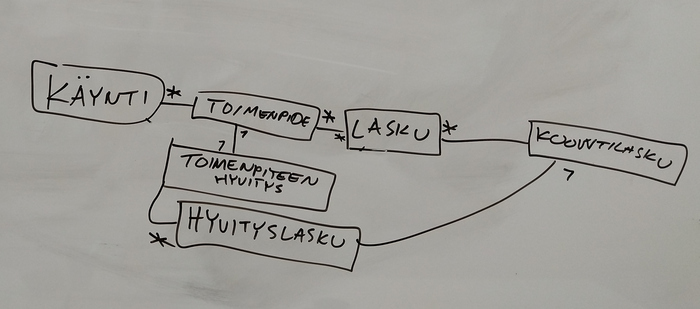
\includegraphics[width=\textwidth,height=0.3\textheight]{illustration/malli1.jpg}
\caption{\label{malli1}: Ensimmäinen malli}
\end{figure}

Oikeastaan käynnillä voi olla monta erillistä asiaa, ne ovat
laskutettavia toimenpiteitä. Palaverin lopuksi aikaansaatu kaavio on
kuvassa \ref{malli1}.

Tämä päätettiin toteuttaa.

Minulla meni torstaisen kokouksen jälkeen perjantai ja maanantai
perusrakenteen pystyttämiseen: Falcon, Ariadne GraphQL, Gunicorn ja
muutamia muita työkaluja. Lisäksi hommasin Pytest-testikirjaston, ja
opiskelin sen.

Lisäksi piti asentaa Apollo GraphQL-client ja Vue-cli, sekä plugin
Vue-Apollo.

Tiistaina sain ensimmäisen toiminnon, käyntien lisäämisen, valmiiksi.

Oli mielenkiintoista huomata, miten piirtämäni kuva ja tässä vaiheessa
aikaansaamani GraphQL-skeema muistuttivat läheisesti toisiaan.
GraphQL-queryjen sisältämät oliot rakensivat saman rakenteen, joka
tussitaululle piirsin. Sen sijaan GraphQL-mutaatioiden rooli ei ole
vielä auennut.

\hypertarget{viikko-2}{%
\section{Viikko 2}\label{viikko-2}}

Ensimmäisellä kehitykseen käyttämälläni viikolla (to-to) sain siis vain
ekan ominaisuuden valmiiksi. Sen jälkeen loppuviikosta tein vielä
käyntien laskutuksen. Lienee rehellistä arvioida, että noin viikon
kehitystyön myötä kaksi ``käyttäjätarinaa'' valmistui.

Perjantaina myös kirjoitin frontendia Vue-Apollolla ja käytin melkoisen
määrän aikaa kirjaston ominaisuuksien hahmottamiseen. Se ei kuulu
suoraan insinöörityön sisältöön, mutta toisaalta kuitenkin tarjoaa hyvän
kehyksen asioiden tekemiseen.

\hypertarget{viikko-3}{%
\section{Viikko 3}\label{viikko-3}}

Sain ensimmäisen version laskuhärvelistä valmiiksi. Tavoite oli Lauran
kanssa pitää asiasta palaveri perjantaina, mutta se peruuntui, koska
Laura oli tulossa kipeäksi.

Laskuhärveli toimii sinänsä, ja on hankala miettiä, onko siitä apua.

Kuitenkin domain-tason konseptien mallintaminen GraphQL-skeemaksi toimii
hyvin. Esimerkki, jossa koontilaskulla (ConsolidatedInvoice) voi olla
monta laskua (Invoice):

\begin{verbatim}
Type Invoice {
  number: Int
  sum: Float
  date: Date
}

type ConsolidatedInvoice {
  number: Int
  invoices: [Invoice]
}
\end{verbatim}

\hypertarget{palaveri-lauran-kanssa-tietomallin-kehittuxe4misestuxe4}{%
\section{27.9.2021 - Palaveri Lauran kanssa tietomallin
kehittämisestä}\label{palaveri-lauran-kanssa-tietomallin-kehittuxe4misestuxe4}}

Esittelin Lauralle tähän asti luomani softaproton. Pääasiallinen ongelma
on mielestäni laskun ja käynnin välisessä yhteydessä. Se, että laitetaan
käynti suoraan laskulle, on ongelmallista. Olin jo pitkin viikkoa
miettinyt, voisiko olla olemassa \textbf{Käyntirivi} ja \textbf{Käynnin
hyvitysrivi}, jotka sijaitsisivat laskulla ja koontilaskulla, ja
kumoaisivat toisensa.

Rupesin piirtämään Lauralle mallia, jossa Käynti liittyy Invoice-olioon,
ja Invoicea vastaa Credit Note, joka kumoaa Invoicella olevia käyntejä.
Piirsin Invoice- ja Credit note -olioiden sisään viivoja edustamaan
näitä käyntejä.

Laura totesi, että oikeastaan kirjanpidon kannalta täytyy täyttyä jokin
\textbf{Laskutusperuste}, jotta asia voidaan laskuttaa. Innostuin tästä
termistä, ja pyysin Lauraa jatkamaan. Laura sanoi, että laskutusperuste
on se, jonka pohjalta voidaan valita asioita laskutettavaksi. Asiat,
jotka täyttävät laskutusperusteen, mutta joihin ei liity laskua, voidaan
esimerkiksi listata laskuttamista varten. Pohjimmiltaan laskutusperuste
voi olla joko tavara tai palvelu, koska niitähän kaikki firmat myyvät.
Valitsimme laskutusperustetta kuvaamaan englanninkielisen termin
\textbf{BasisForInvoicing}. Palvelu on \textbf{Service}.

Ehdotin mallia, jossa \textbf{Appointment} voidaan viedä
\textbf{Invoicelle} \textbf{ServiceRow}-olioksi, jos täyttyy
BasisForInvoicing-ehto. Laura kurtisteli kulmiaan, eikä sanonut mitään.
Kysyin siis, eikö malli oikein miellytä, ja Laura totesi, että se
näyttää liian monimutkaiselta.

Pyyhin taulun puhtaaksi, ja kokeilimme uudestaan. Tein \textbf{Invoice}
-olion, jonka alle laitoin \textbf{ServiceRow} -nimisen olion. Invoicea
vastaamaan piirsin \textbf{CreditNote} -olion, jonka alle
\textbf{ServiceCreditRow}. Sivummas piirsin Appointment-olion, ja
pohdimme, mikä sen suhde voisi olla laskutukseen.

\begin{figure}
\centering
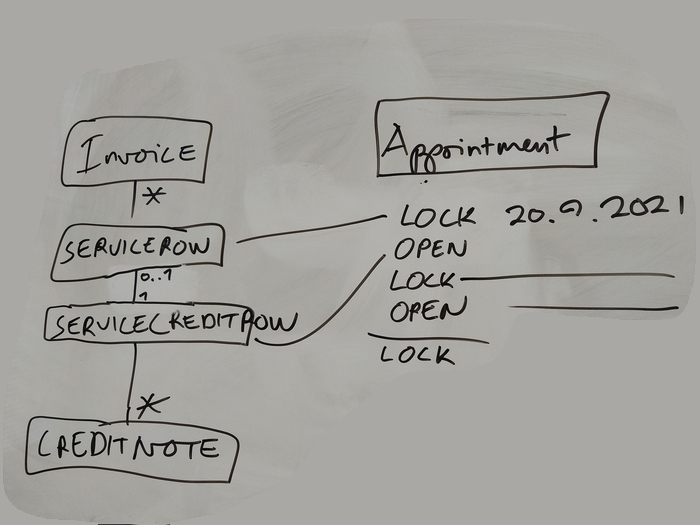
\includegraphics[width=\textwidth,height=0.5\textheight]{illustration/malli2.jpg}
\caption{\label{malli2}Toinen malli}
\end{figure}

Yhtäkkiä minulla välähti: mitä, jos tehtäisiin ikäänkuin loki
\textbf{Appointment}-olion sisälle: sinne tallennettaisiin
lukitustapahtuma, kun \textbf{Appointment} liitetään laskulle luomalla
sitä vastaava \textbf{ServiceRow}. Ja vastaavasti kun
\textbf{ServiceRow} hyvitettäisiin \textbf{ServiceCreditRown} avulla,
voitaisiin luoda avaustapahtuma. Näin ollen \textbf{Appointment}-luokan
alla olisi lista tapahtumia, ja listan avulla nähtäisiin sekä
laskutushistoria, että myös käynnin tämänhetkinen laskutustilanne:
Laskuttamatta vai avoinna? Esitän mallin kuvassa \ref{malli2}.

Laura huomautti, että tämä ei kuitenkaan ratkaise sitä pääongelmaa, joka
meillä on ollut: että käynnin hinta pitäisi jakaa monelle eri
maksajalle, joille lähetettyjä laskuja on voitava hyvittää itsenäisesti.

Niinpä pyyhin taas koko taulun puhtaaksi, ja lähdimme taas uudelleen
liikkeelle.

Nyt Käynnin alle lisättiin erillinen, laskutustarkoituksiin käytettävä
olio, jonka nimeksi pistettiin \textbf{BasisForInvoicing}. Tämä
BasisForInvoicing voidaan jakaa osiin, ja jokainen osa sisältää oman
erillisen listansa laskutustapahtumista: onko osa liitetty laskuun, vai
onko se hyvitetty ja taas siis avoinna.

\begin{figure}
\centering
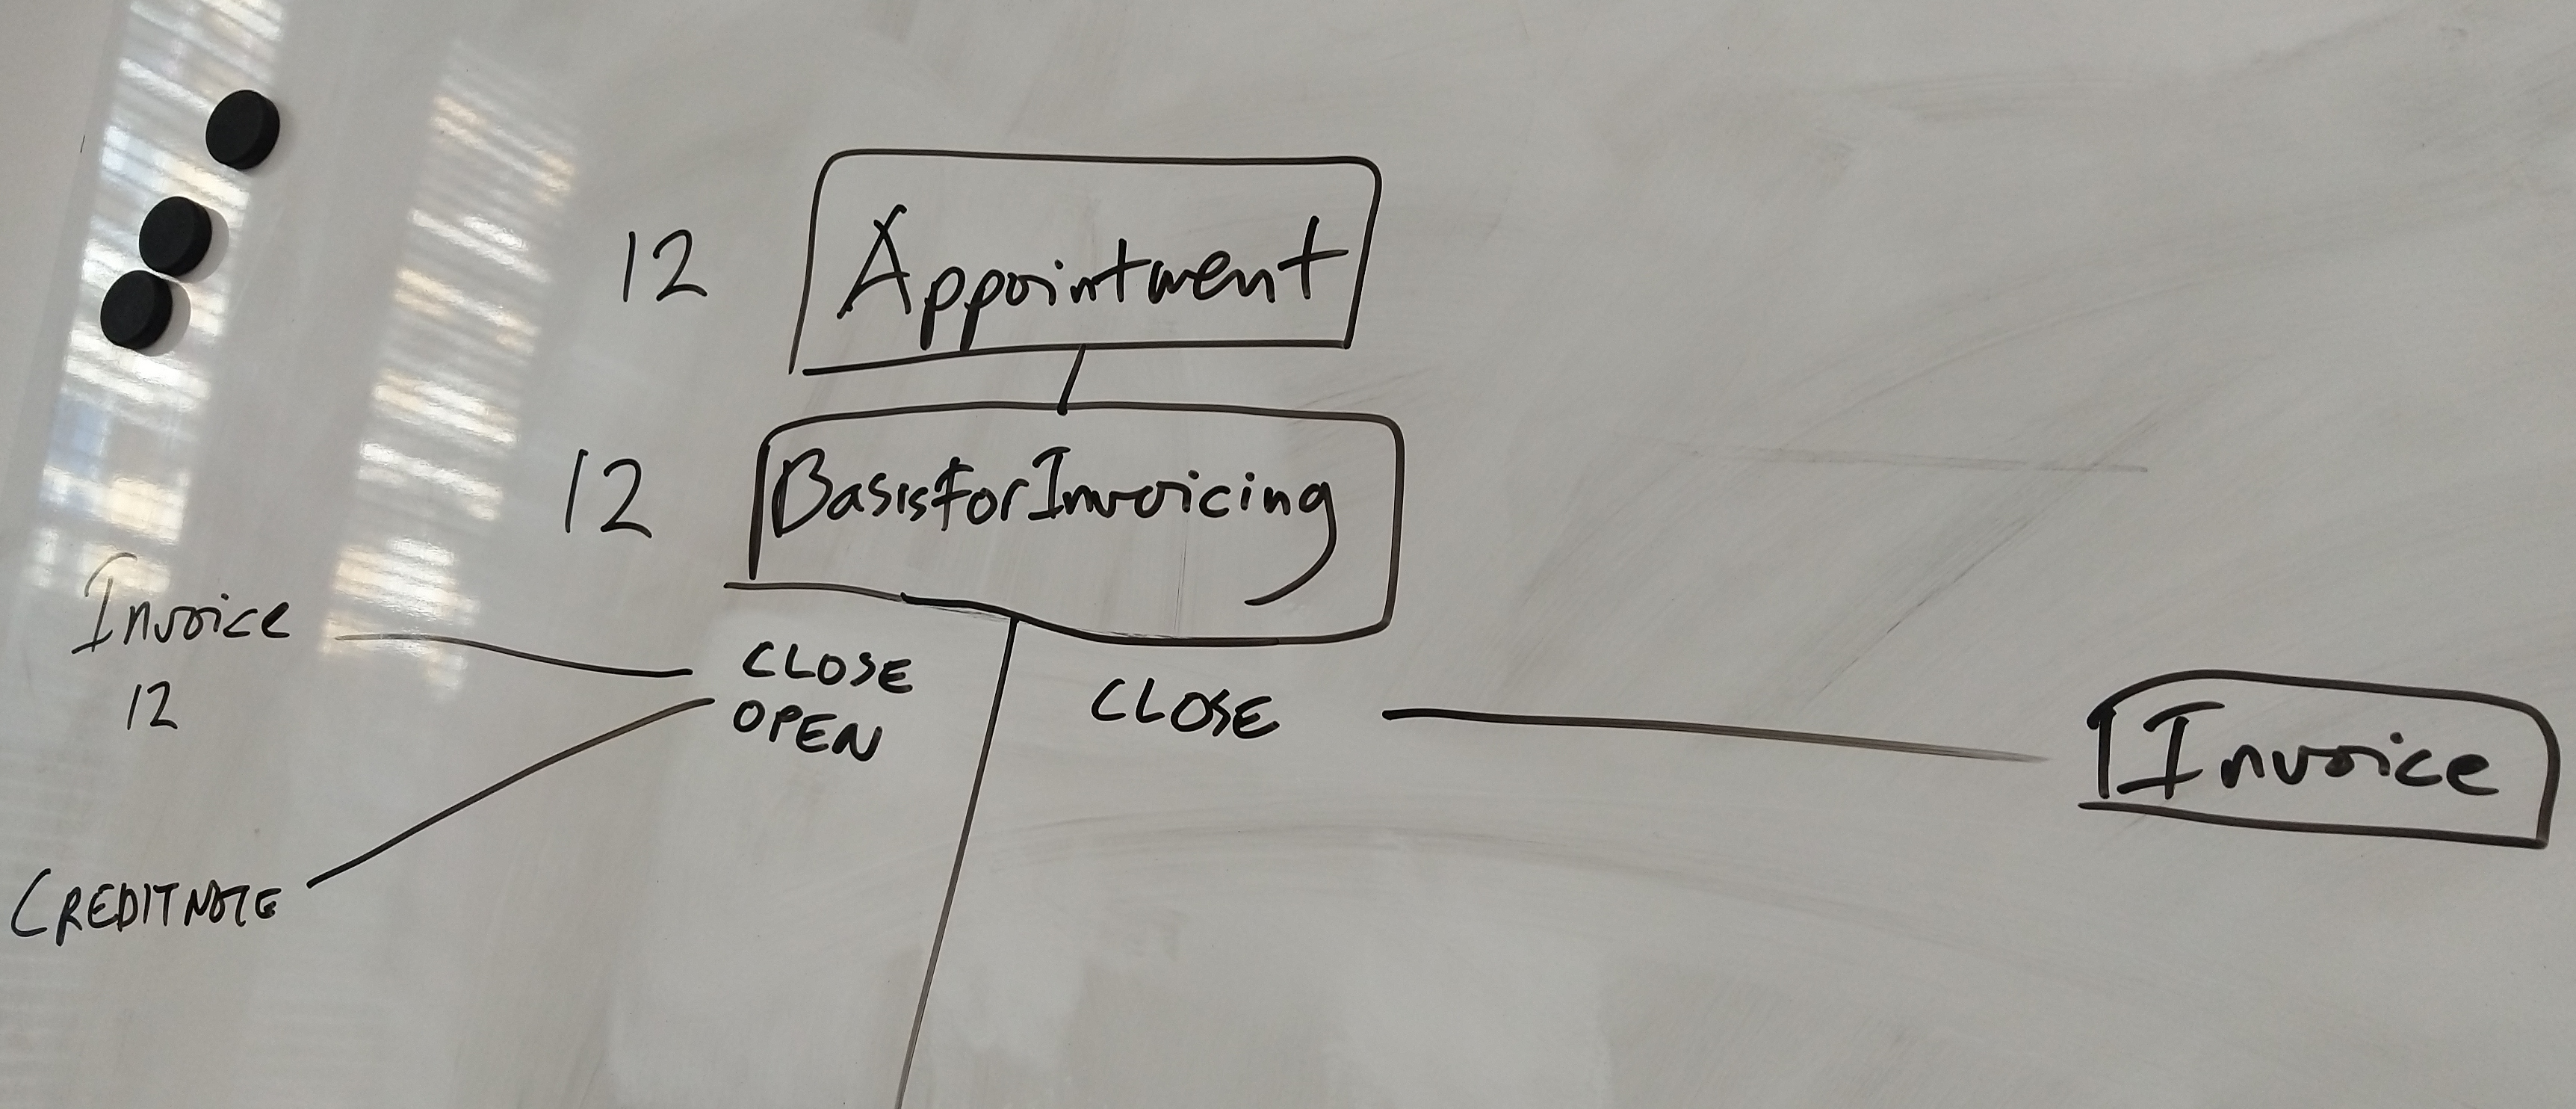
\includegraphics[width=\textwidth,height=0.5\textheight]{illustration/malli3.jpg}
\caption{\label{malli3}Kolmas malli}
\end{figure}

Tämä tuntui meistä hyvältä mallilta, ja sen pohjalta ryhdyin koodaamaan.
Tätä mallia esittää kuva \ref{malli3}. Sovittiin uusi palaveri viikon
päähän.


% Sample content to demonstrate LaTeX command. You will likely delete this line and the
% next \input{sample/*} lines. You are also safe to delete the sample/ folder and its
% content once you refershed your LaTeX skills. Also check the appendix samples.
% \input{sample/1content.tex}
% \input{sample/2lorem.tex}
% \input{sample/3graph.tex}

%----------------------------------------------------------------------------------------
%	BIBLIOGRAPHY REFERENCES
%----------------------------------------------------------------------------------------

\input{style/biblio.tex}

%----------------------------------------------------------------------------------------
%	APPENDICES
%----------------------------------------------------------------------------------------

\input{style/appendix.tex}
%force smaller vertical spacing in table of content
%!!! There can be some fun depending if the appendices have (sub)sections or not :D
% You will have to play with these numbers and eventually add the \vspace line  before
% some \chapter and force another number.
% To add more fun, time to time the table of content get wrong after a build :(
\addtocontents{toc}{\vspace{11pt}}
\pretocmd{\chapter}{\addtocontents{toc}{\protect\vspace{-24pt}}}{}{}

\liite{1}% This is a hack to have right page numbering for each appendix. Make sure to
% use a unique number for each appendix.
\input{sample/Xappendix1.tex}% Sample content to demonstrate appendix in LaTeX. You
% are safe to delete this lines (and the next samples) once you refreshed your LaTeX
% skills (and safe to delete the sample folder and all its file too).

%\addtocontents{toc}{\vspace{11pt}}%fix vertical space for Table of Content
\liite{2}
\input{sample/Xappendix2.tex}

\addtocontents{toc}{\vspace{11pt}}
\liite{3}
\input{sample/X_R_example.tex}


%----------------------------------------------------------------------------------------
%	THIS IS THE END
%----------------------------------------------------------------------------------------
\end{document}
